
\FloatBarrier

\section{Recover a correspondence with extra intermediate points}

We build a grammar from a single example from the hand-annotated Romer
dataset, and use it to parse a curve from the ground-truth Romer
dataset. We successfully recover a very reasonable correspondence.

\begin{figure}
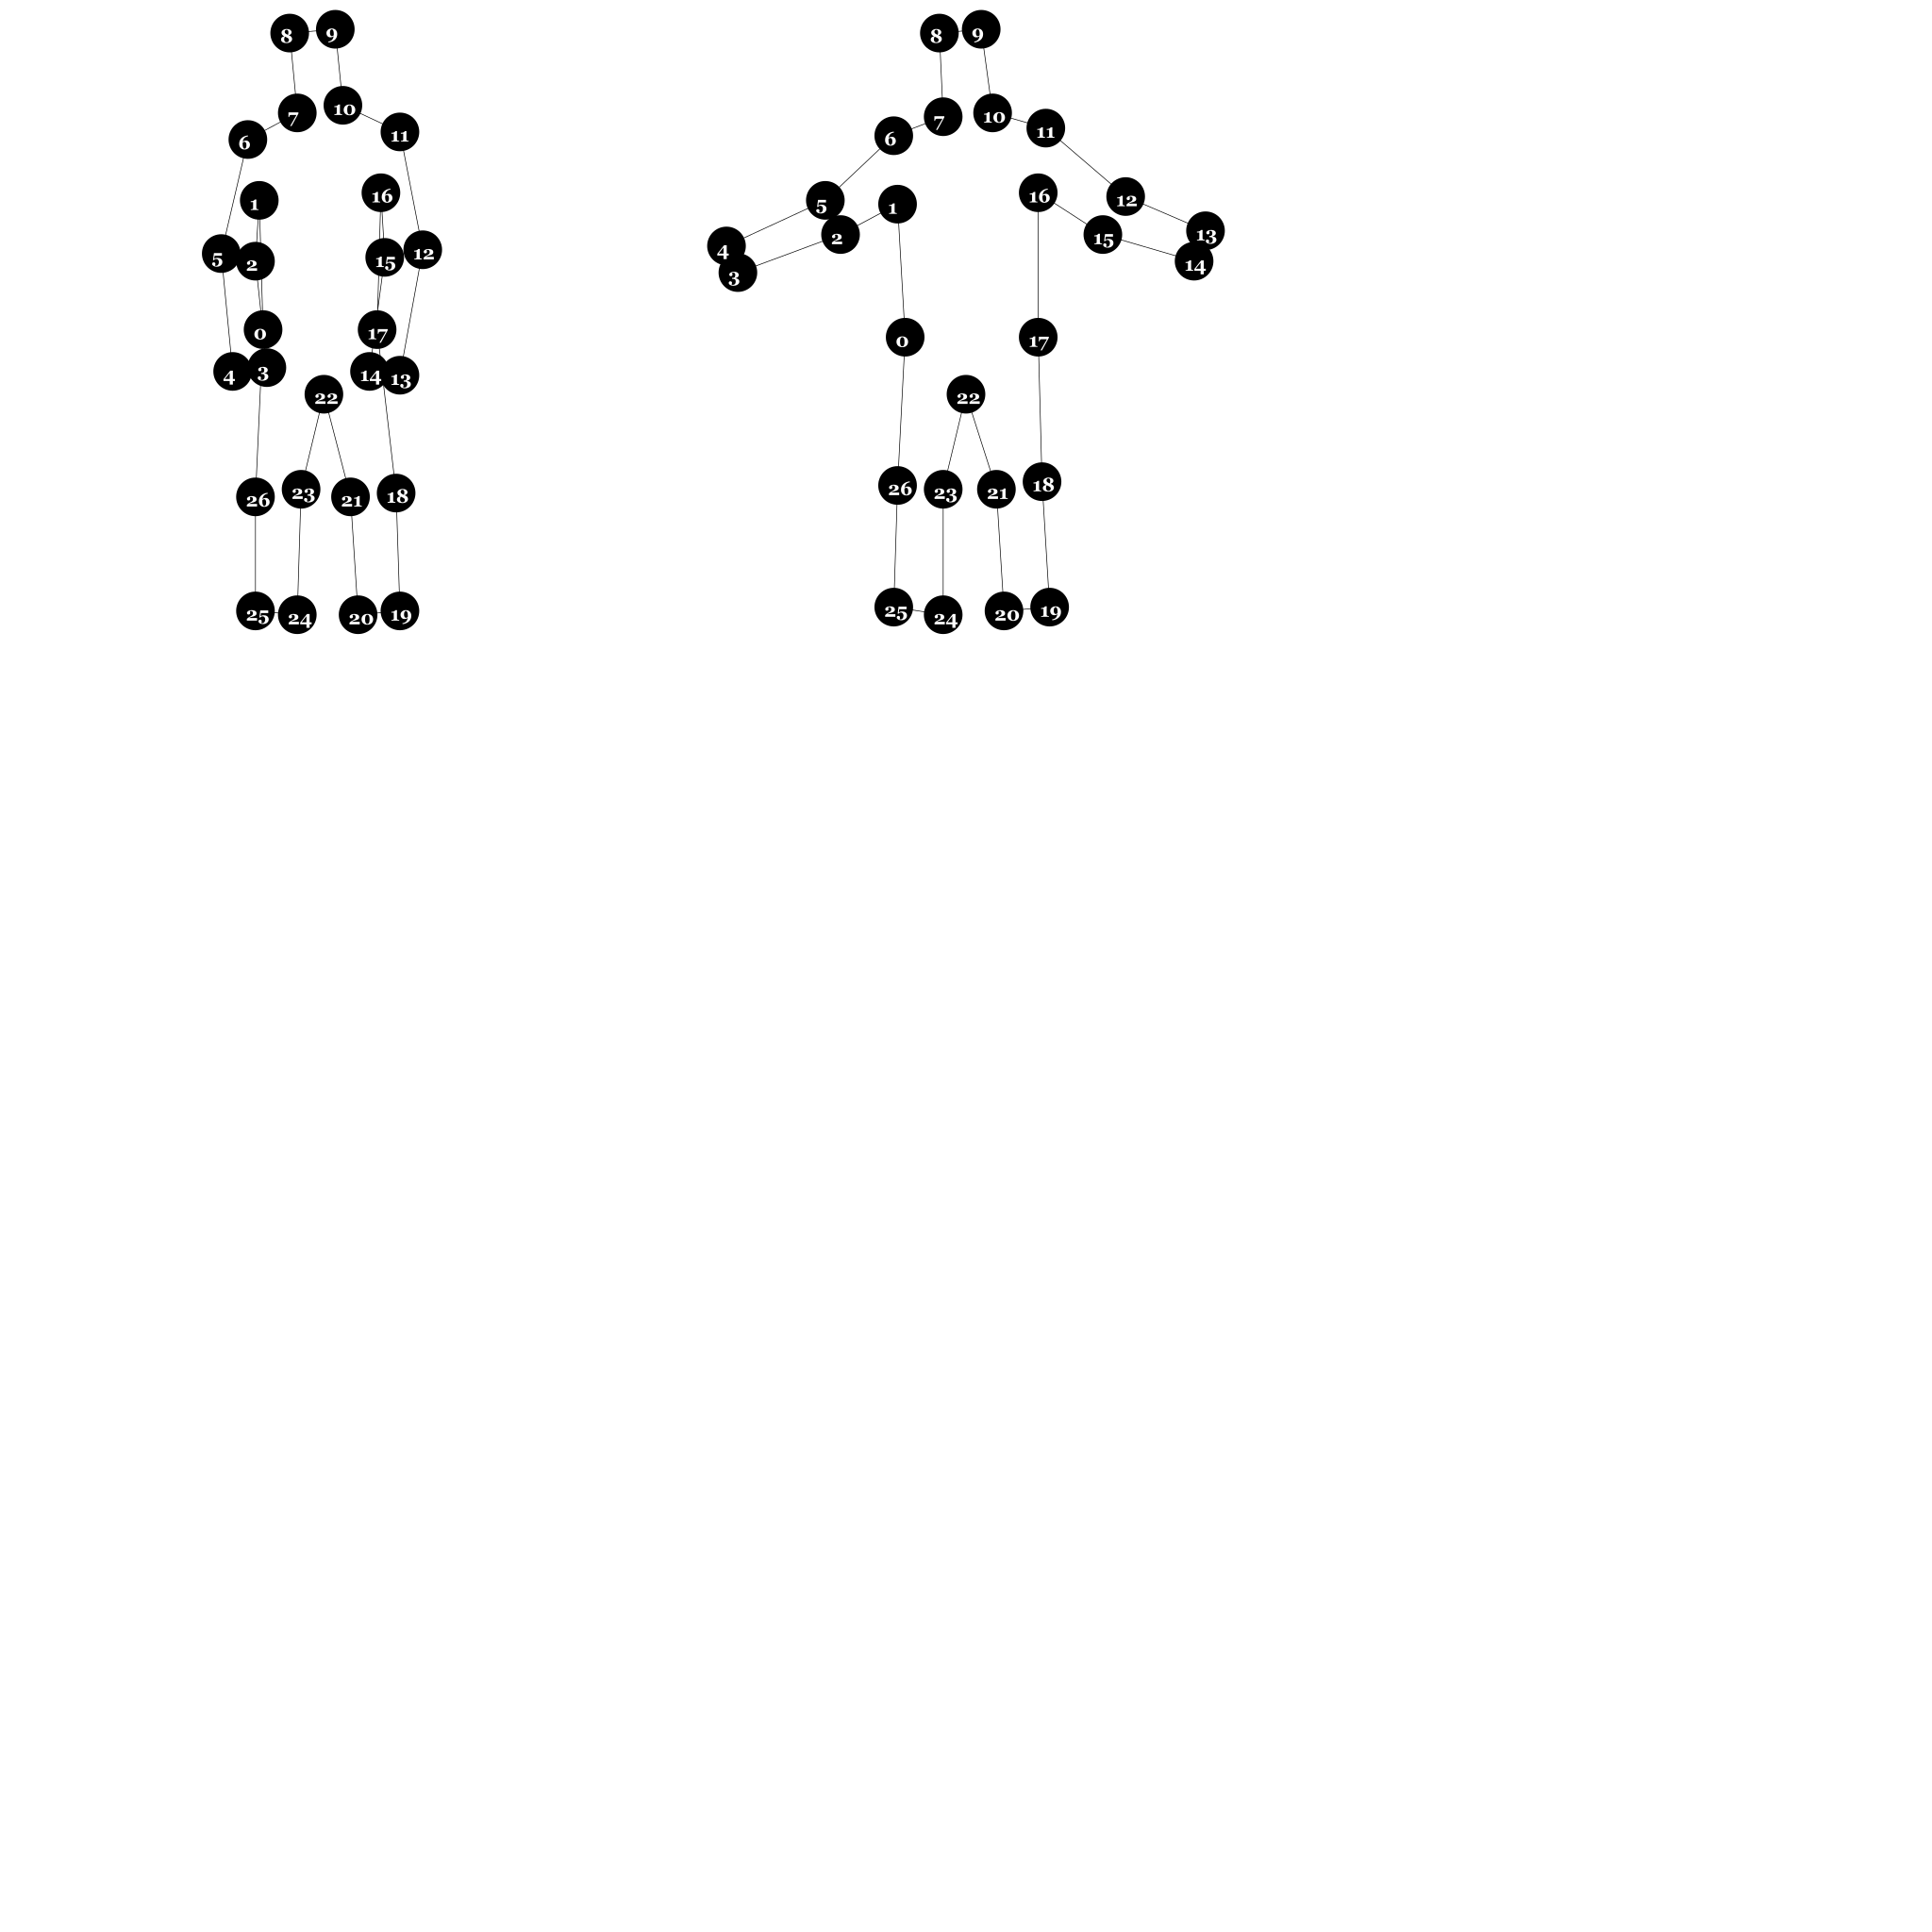
\includegraphics[width=\linewidth]{experiments/2.parsing/longer_curves/output.d/parse.png}
\caption{On the left, the model curve. On the right, the parsed curve}
\end{figure}

The ground-truth Romer curve has more intermediate points, so this
demonstrates that our grammar construction and parsing algorithm deal
well with additional intermediate points. The grammar must have
lengthening rules, but doesn't need shortening rules.

